\chapter{Visual Analytics of Spatiotemporal Social Media for Abnormal Event Detection}

%Many social media services have emerged in the past years 
%and they provide different types of information according to the purpose of the services.
Social media services, e.g, Twitter, Youtube, Flickr, provide a rich and freely accessible 
database of user-generated situation reports. As advances in technology have enabled
%and the user information tends to contain mainly 
%user's spatial and temporal information while the social media content is being generated.
%Since smart mobile devices became popular recently,
%it is even easier to produce lots of social media data anywhere and anytime. 
%mobility of the 
the widespread adoption of GPS enabled mobile communication
devices, these reports are able to capture important local events observed by an active and ubiquitous community.
The different forms of social media content provided by the users,
such as microposts, images or video footage, can have immense value 
for increasing the situational awareness of ongoing events.

% However, as data volumes have increased beyond the capabilities of manual evaluation, 
% there is a need for advanced tools %plays an important role to provide
% as a means to provide insights for investigation and to understand the extent, 
% severity and consequences of incidents, as well as their time-evolving nature.
% Due to the large number of individual social media messages it is not straightforward 
% to analyze and extract meaningful information. 
% For example, in Twitter, more than 200 million Tweets are posted each day~\cite{Tweets:2011:Twitter}.
% %and a billion Tweets are created
% %every five days as of June 30, 2011.
% Thus, in an ongoing scenario, the relevant messages for situational awareness are usually buried by
% a majority of irrelevant data. 
% Finding and examining these messages without smart aggregation, automated text analysis and 
% advanced filter strategies is almost impossible and extracting meaningful information is even more challenging.

However, as data volumes have increased beyond the capabilities of manual evaluation, there is a need for
advanced tools to aid understanding of the extent, severity and consequences of incidents, 
as well as their time-evolving nature, and to aid in gleaning investigative insights. 
Due to the large number of individual social media messages it is not straightforward to analyze and extract meaningful information. 
For example, in Twitter, more than 200 million Tweets are posted each day~\cite{Tweets:2011:Twitter}. 
Thus, in a developing event, the relevant messages for situational awareness are usually buried by a majority of irrelevant data. Finding and examining these messages
without smart aggregation, automated text analysis and advanced filtering strategies is almost impossible and
extracting meaningful information is even more challenging.

%Another issue is reliability of the data.
%Posts might be outdated, incorrect, or simply unimportant
%and this can heavily interfere with searching for meaningful information. 
%Previously researchers have focused
%on finding spatial and temporal trends according to volume-based importance.
%In other words, a large volume of keywords or content is considered to be more important.
%This type of analysis can cause relatively small volumes of important data to be easily obscured.
%by huge amount of data
%which tends to indicate normal situations, but
%abnormality within a small volume of data can provide more critical and important information for unusual events.

To address these challenges, we present an interactive spatiotemporal social media analytics approach
for abnormal topic detection and event examination~\cite{CHAE:2012:SSM}.
In order to find relevant information within a user defined spatiotemporal frame
%within the social media data, 
we utilize the LDA topic model~\cite{Blei:2003:LDA}, which extracts 
and probabilistically ranks major topics contained in textual parts of the social media data.
%The abnormality is estimated from the major topical events.
The ranks of the categorized topics generally provide a volume-based importance,
but this importance does not reflect the abnormality or criticality of the topic. 
In order to obtain a ranking suitable for situational awareness tasks, we discard daily chatter
by employing the STL~\cite{Cleveland:1990:SAS}.
%based on the abnormality estimation.
In our work, globally and seasonally trending portions of the data are considered less important,
whereas major non-seasonal elements are considered anomalous and, therefore, relevant.

However, due to the large volumes of data, the very specific syntax and semantics of microposts and 
the complex needs of situational analysis, it would not be feasible to apply these techniques 
in the form of a fully automated system. 
Therefore, our whole analysis process, including the application of automated tools, is guided and 
informed by an analyst using a highly interactive visual analytics environment. 
It provides tight integration of semi-automated text-analysis and probabilistic event detection tools 
together with traditional zooming, filtering and exploration following the Information-Seeking Mantra~\cite{Shneiderman:1996:TEH}.

%We apply our techniques to various social media data sources, including Twitter, Flickr, and YouTube,
%to improve reliability of the 
%as a way of testing our abnormality detection scheme. 
%Moreover, it is possible to compare and analyze which information users post according to
%the social media services.
%Finally, our geovisual analytics system is used for situational awareness of
%abnormality within social media data and enables a scalable
%visual examination and highly interactive visual analysis workbench for spatiotemporal trend analysis.
%interactive capability of spatiotemporal trend analysis. 
%The remainder of this document is structured as follows: 
%Section~\ref{sec:relatedwork} is a review of related work.
%The automated methods to find and examine unusual topics and events are described in Section~\ref{sec:social_analytics}.
%In Section~\ref{sec:analysisprocess} we briefly introduce our visual analytics system Scatterblogs, which was already featured in previous works, and explain how the automated methods are integrated within a sophisticated iterative analysis loop.
%Finally we demonstrate the performance of our system based on selected case studies in Section~\ref{sec:case_study} and discuss the approach in Section~\ref{sec:disc}.

\section{Spatiotemporal Social Media Analytics for Event Examination}
\label{sec:social_analytics}
Since several social media sources recently provide space-time indexed data, traditional techniques for spatiotemporal zooming, filtering and selection can now be applied to explore and examine the data.
However, as message volumes exceed the boundaries of human evaluation capabilities, it is almost impossible to perform a straightforward qualitative analysis of the data.
In order to cope with the data volumes, traditional interaction and visualization techniques have to be enhanced with automated tools for language processing and signal analysis, helping an analyst to find, isolate and examine unusual outliers and important message subsets.

To address this issue, we present an interactive analysis process that integrates advanced techniques for automated topic modeling and time series decomposition with a sophisticated analysis environment enabling large scale social media exploration. 
In part~\ref{subsec:topic_extraction} of this Section we first explain how the Latent Dirichlet Allocation, a well established topic modeling technique in the information retrieval domain, can be used to extract the inherent topic structure from a set of social media messages. The output of this technique is a list of topics each given by a topic proportion and a set of keywords prominent within the topics messages. In a subsequent step, our system then re-ranks the retrieved topic list by identifying unusual and unexpected topics. This is done by employing a seasonal-trend decomposition algorithm to the historic time series data for each topic, retrieving its seasonal, trending and remainder components. 
Using a z-score evaluation, we locate peaks and outliers in the remainder component in order to find an indicator of unusual events.
While the LDA topic extraction is done primarily for Twitter data, 
the abnormality estimation is also applied to different social media data sources, such as Flickr and YouTube, for each topic. 
This is achieved by searching matching entries for each term of a topic and applying the same STL analysis on the resulting time series.
The results are available to the analyst for cross validation.
The details of this step are described in Subsection~\ref{subsec:filtering} and the complete detection model is formally described in Subsection~\ref{subsec:analysis_multi_social}. In Section~\ref{sec:analysisprocess}, 
we describe how powerful tools based on these techniques are used within our analysis environment, Scatterblogs, 
in order to iteratively find, isolate and examine relevant message sets.

%~\ref{fig:process}.

%Our main goal is identifying such unusual and even critical events within the social media data set.
%We carried out a series of experiments to extract topics from Tweets in 7 days prior to the event date.
%In result, the common topics had large proportion values for almost every day, but there was not the abnormal 
%event topic in the experimental results.
%As we were motivated by this experimental result, 
%
%first, we sampled Tweets that include 
%at least one of the words of individual topics and generate time series of daily count Tweets per topic.


%\textbf{Visualization:}
%Our system provides an interactive scalable geo-locational visualization using the ranked abnormal topics
%by plotting the locations of the social media data referring the topic and displaying term clouds of the topic words.
%Moreover, the system enables an iterative analysis of the data through user interaction.

%assume abnormal events rarely occur
%We focus on such unusual topics and events

%% \subsection{Data collection}
%% \label{subsec:data_collection}

%% \section{Abnormal event and topic detection}
%% \label{sec:abnormal_dect}

%%

\subsection{Topic Extraction}
\label{subsec:topic_extraction}

\begin{table}[b]%\footnotesize
\begin{center}
\begin{tabular}{|l|l|l|}
	\hline
	 Rank & Proportion & Topics \\
	\hline\hline
	1 & 0.10004  & day back school today \\ %work \\
	2 & 0.09717	 & lls bout dat wit \\ %yea \\
	3  & 0.09443 & people make hate wanna \\ %life  \\
	4 & 0.08226 & \textbf{earthquake thought house shaking} \\ %damn}  \\
	5 & 0.05869 & \textbf{earthquake felt quake washington} \\ %virginia} \\	
	\hline
\end{tabular}
\caption{An example of extracted topics and their proportions.
We extracted topics from Tweets written on August 23, 2011 around Virginia, 
where an earthquake occurred on this day.
One can see that topics consisting of ordinary and unspecific words can have high proportion values,
while the earthquake related topics have a relatively low proportion value.}
\label{T:TopicProportion}
\end{center}
\end{table}


%\begin{table*}[t]\footnotesize
%\begin{tabular}{|c|c|c|}
	%\hline
	%\multicolumn{3}{|c|}{Number of Iteration Steps in the LDA process}\\
	%\hline
	%50 & 300 & 1000 \\
	%\hline\hline
	%foursquare pic hall brooklyn & time back night day  & time night nyc day   \\
	%time night day back  & york ave brooklyn btw  & york ave brooklyn park  \\
	%newyork nyc tweetmyjobs finance  & pic bar food nyc  & \textbf{foursquare occupywallstreet  mayor ousted} \\
	%york brooklyn ave street  & \textbf{foursquare occupywallstreet park mayor}  & newyork tweetmyjobs finance citigroup  \\
	%york ave park btw 	& newyork tweetmyjobs finance citigroup  & \textbf{san gennaro street italy}   \\
	%\hline
%\end{tabular}
%\caption{An example of topic model results depending on the number of iteration steps in the LDA process.
%The topics are extracted from the Tweets posted in New York City on September 17 and 18, 2011 where the Occupy Wall Street protest movement began and
%a famous festival, \textit{San Gennaro} occurred.
%A higher number of sampling iterations provides a better topic retrieval describing the two different events.}
%\label{T:TopicResults}
%\end{table*}

Our monitoring component collects space-time indexed Twitter messages using the Twitter-API.
The received messages are preprocessed and then stored in our local database.
When users of these services witness or participate in unusual situations 
they often inform their friends, relatives or the public about their observations.
%Often when an unusual situation happens 
%or a controversial issue comes out in a social 
%environment, 
%a certain number of messages
%will be generated about the event or the topic within the social network.
%it depends on the total number of sampled messages (e.g., a couple of hundreds, thousands or more), 
%rather than an individual post, 
%
If enough users participate, the communication about the situation constitutes a topic that makes up a certain proportion of all messages within the database, or some messages within a predefined area and timespan.
In most cases, however, the proportion will be smaller than that of other prevalent topics, such as discussions about movies, music, sports or politics.
In order to extract each of the individual topics exhibited within a collection of social media data, 
we employ Latent Dirichlet Allocation, a probabilistic topic model that can help organize, understand, and summarize vast amounts of information.
%The detail of this \textit{topic extraction} is presented in Section~\ref{subsec:topic_extraction}.

The LDA topic model approach, as presented by David Blei et al.~\cite{Blei:2003:LDA}, 
is a probabilistic and unsupervised machine learning model to identify latent topics and corresponding document clusters from a large document collection.
Basically, it uses a \textquotedblleft bag of words\textquotedblright approach and assumes that a document exhibits multiple topics 
distributed over words with a Dirichlet prior. 
In other words, the LDA assumes the following generative process for each document: 
First, choose a distribution over topics, choose a topic from the distribution for each word,
and choose a word associated with the chosen topic.
Based on this assumption one can now apply a Bayesian inference algorithm to retrieve the topic structure of the message set together with each topic's statistical proportion and a list of keywords prominent within the topic's messages.
Table~\ref{T:TopicProportion} shows an example set of extracted topics resulting from the application of LDA to Twitter data ordered by the proportion ranking. The example social media data was collected from Twitter for the Virginia area on August 23rd.
On this day, the area was struck by an earthquake with a magnitude of 5.88.
As seen in the table, this earthquake event was captured as a topic within the Twitter messages.
%First, users select a large collection of Twitter messages for a target area and a time period.
%Given the messages, the LDA topic modeling procedure extracts a set of topics.
%Each topic is a set of words, which are associated with a corresponding topic.
% The LDA is a probabilistic and statistical model to identify latent topics from a large 
% document collection, which was presented as a topic model by David Blei et al.~\cite{Blei:2003:LDA}. 
% Basically, this topic model assumes that a document exhibits multiple topics 
% distributed over words in the document.
% Recently, researchers applied the topic model to social media data to summarize 
% and categorize Tweets~\cite{Zhao:2011:CTA} and find influential Twitters~\cite{Weng:2010:TFT}. 
% Zhao et al.~\cite{Zhao:2011:CTA} demonstrate characteristics of Twitter by comparing the content 
% of Twitter with a traditional news medium like New York Times.
% They also propose a different Twitter-LDA model and compare the new model with the standard model and 
% %a different topic model named 
% with the author-topic model~\cite{Steyvers:2004:PAM}.
% In the author-topic model, a document is assumed to be a topic mixture by multiple authors.
% In this work, we use the standard LDA model since a single message is generated by a single user.
% %~\cite{Weng:2010:TFT, Hong:2010:EST} used the author-topic model to discover topics from Tweets.
% ParallelTopics~\cite{Wenwen:2011:PAP} also extracts meaningful topics using LDA from a collection of documents.
% The visual analytics system allows users to interactively analyze temporal patterns of 
% the multi-topic documents.

In our system, the MALLET toolkit~\cite{McCallum:2002:MALLET} is used for the topic analysis.
%If not noted otherwise, 20 topics and 1000 iterations were used for the result presented in this work.
Prior to the topic extraction, the stemming algorithm KSTEM by Krovetz~\cite{Krovetz} is applied to every term in the messages.
The results of KSTEM are more readable and introduce fewer ambiguities than the often used Porter stemmer.

\begin{table}[ht]%\footnotesize
\begin{center}
\begin{tabular}{|c|}
	\hline
	Number of Iteration Steps in the LDA process\\
	\hline
	50 \\
	\hline\hline
	foursquare pic hall brooklyn \\
	time night day back \\
	newyork nyc tweetmyjobs finance \\
	york brooklyn ave street \\
	york ave park btw \\
	\hline
	300 \\
	\hline\hline
	time back night day \\
	york ave brooklyn btw
	pic bar food nyc \\
	\textbf{foursquare occupywallstreet park mayor} \\
	newyork tweetmyjobs finance citigroup \\
	\hline
	1000 \\
	\hline\hline
	time night nyc day   \\
	york ave brooklyn park  \\
	\textbf{foursquare occupywallstreet  mayor ousted} \\
	newyork tweetmyjobs finance citigroup  \\
	\textbf{san gennaro street italy}   \\
	\hline
\end{tabular}
\end{center}
\caption{An example of topic model results depending on the number of iteration steps in the LDA process.
The topics are extracted from the Tweets posted in New York City on September 17 and 18, 2011 where the Occupy Wall Street protest movement began and
a famous festival, \textit{San Gennaro} occurred.
A higher number of sampling iterations provides a better topic retrieval describing the two different events.}
\label{T:TopicResults}
\end{table}

For the unsupervised LDA classification and topic retrieval one has to define two parameters: the number of expected topics and the number of iterations for the Gibbs sampling process~\cite{Griff:2004:FST}, which is used in MALLET for the topic inference.
The number of topics that should be chosen depends on the size of the document collection and the 
required overview level. A small number of topics (e.g., 10) will provide a broad overview of the documents, whereas
a large number (e.g., 100) provides fine-grained results.
The number of sampling iterations is a trade-off between computation time and 
the quality of discovered topics.
To illustrate this, Table~\ref{T:TopicResults} shows the experimental results of the topic model using a varying number of sampling iterations while the number of topics was set to four.
The topics were extracted from Tweets posted in New York City
on September 17 and 18, 2011, where a large group of protesters occupied Wall Street in New York City. 
%This event began September 17, 2011.
A topic indicating the Occupy Wall Street protests can be seen when using at least 300 iterations. At the time of these protests, there was also a famous annual festival, the \textit{San Gennaro}, occurring in Little Italy. This can only be seen when using at least 1000 iterations.
As shown in Table~\ref{T:TopicResults}, the topics with 50 iterations do not indicate any meaningful events.
The topics with 300 iterations, on the other hand, consist of more distinguishable classes.
Finally, the topics with 1000 iterations obviously point out individual events which happened in the city.



%	foursquare pic hall brooklyn mayor & time back night day people & time night nyc day back  \\
%	time night day back people & york ave brooklyn btw street & york ave brooklyn park btw \\
%	newyork nyc tweetmyjobs finance citigroup & pic bar food nyc brunch & foursquare occupywallstreet pic mayor ousted \\
%	york brooklyn ave street city & foursquare occupywallstreet park mayor island & newyork tweetmyjobs finance citigroup citijobs \\
%	york ave park btw broadway	& newyork tweetmyjobs finance citigroup citijobs & san gennaro street italy york  \\
%\subsection{Filtering unusual events and topics}
\subsection{Abnormality Estimation using Seasonal-Trend Decomposition}
\label{subsec:filtering}
Abnormal events are those that do not happen frequently and usually they cover only a small fraction of the social media data stream.
As shown in Table~\ref{T:TopicProportion}, even during an earthquake episode, highly ranked topics consist of ordinary and unspecific words.
The third and fourth ranked topics include words indicating the earthquake event of August 2011:
\textit{earthquake felt quake washington}.
%In the analysis of social media data, one of the most challenging problems is the extraction of 
%valuable and critical information as the size of data and the quality of the information 
%have high variance~\cite{Agichtein:2008:FHC}. 
%drastically vary according to users~\cite{Agichtein:2008:FHC}. 
%In addition, a relatively small subset within the data may be easily obscured by large subsets,
%although the smaller subset contains valuable information.
%Table~\ref{T:TopicProportion} shows the extracted topics from Tweets written during the event date, 
%August 23rd 2011 when an earthquake struck the Virginia area.
%We carried out a series of experiments to extract topics from Tweets in the seven days prior to the event date.
%We found that common topics, such as \textit{day back school today},  
%still made a majority of the data over the seven days,
%and there were no topics related to the earthquake event.
From this observation in the distributions of ordinary and unusual topics over the social media data,
it is necessary to differentiate the unusual topics from the large number of rather mundane topics.
In order to identify such abnormal topics, %indicating unexpected situations and unusual social issues,
we utilize the STL~\cite{Cleveland:1990:SAS}.
For each extracted topic of the LDA topic modeling, our algorithm retrieves messages associated with the topic and then generates a time series consisting of daily message counts from their timestamps.
%and discard regular trend and seasonal components.
%we generate a time series for the each topic. 
%
The time series can be considered as the sum of three components: a trend component, a seasonal 
component, and a remainder:
%
\begin{equation}
Y = T + S + R
%Y_t = T_t + S_t + R_t
\end{equation}
%
Here $Y$ is the original time series of interest, 
%where for the day $t$, $Y_t$ is the original time series of interest, 
%(in our case the amount of messages belonging to the extracted topic on day $t$)
$T$ is the trend component,
$S$ is the seasonal component,
and $R$ is the remainder component.
%
%repetition
%The STL decomposes a time series into these separated components using the Loess smoothing technique, 
%which was developed by Cleveland~\cite{Cleveland:1979:RLW} and it has been widely used in time varying data analysis.
STL works as an iterative nonparametric regression procedure using a series of Loess smoothers~\cite{Cleveland:1979:RLW}.
%The nature of STL allows us to robustly mode the time series, account for the various components, 
%and diagnose the irregular component. 
The iterative algorithm progressively refines and improves the estimates of the trend 
and the seasonal components.
The resulting estimates of both components are then used to compute the remainder:
$R = Y - T - S$.
%$R_t = Y_t - T_t - S_t$.
%\textbf{Control chart based abnormality determination:}
Under normal conditions, the remainder will be identically distributed Gaussian white noise, while a large value of $R$ indicates substantial variation in the time series. 
Thus, we can utilize the remainder values to implement control chart methods detecting anomalous outliers 
within the topic time series.
We have chosen to utilize a seven day moving average of the remainder values to calculate the z-scores, 
$z = (R(d) - mean)/std$, where $R(d)$ is the remainder value of day $d$, $mean$ is the mean remainder value for the last seven days, and $std$ is the standard deviation of the remainders,
with respect to each topic.  
If the z-score is higher than 2, events can be considered as abnormal within a 95\% confidence interval.
The calculated z-scores are thus used as abnormality rating and the retrieved topics will be ranked in the analytics environment according to this estimate.
%However, in this scheme, new topics do not have enough data to extract z-scores.  Thus, brand new topics are moved to the top of the topic stream list as they may also be important for the analyst.

%In order to stabilized, improve the interpretability, and appropriately model the time series
%using STL, a power transformation is applied.
%In analysis of the data, we used the logarithm transformation, which is widely used 
%for positive time series data.
%[To do: How to set the parameters in using STL]
%[To do: our results and description]

%\subsection{Anaysis of multipe social media data}
\subsection{Detection Model}
\label{subsec:analysis_multi_social}
To conclude this section, we formalize our abnormal event detection model based on the probabilistic topic extraction and time series decomposition.

An abnormal event is associated with a set of social media messages that provides
its contents, location, and time-stamp.
To detect abnormal events for a given area and timespan,
we define a set called \textit{social spacetime} as follows:
\begin{equation}
S = (T, \Delta{time}, \Delta{area}, msgs)
\end{equation}
where $T$ is a set of topics,
$\Delta{time}$ is a time period (e.g., one day),
$\Delta{area}$ is a bounded geographical region, 
and $msgs$ is a set of messages.
The user selected parameters $\Delta{area}$ and $\Delta{time}$ define the analysis context for which all messages are loaded into the analysis system.
In this context, the user selects a subset of messages ($msgs$) for which the LDA topic modeling procedure (described in Section~\ref{subsec:topic_extraction}) extracts the set of topics, $t_i \in T$. 
Each topic is defined as:
\begin{equation}
t_i = (M_i, W_i, z_i, Y_i, p_i)
\end{equation}
where 
$W_i$ is a set of words describing the topic, 
$M_i$ is a set of relevant messages,
$z_i$ is an abnormality score (z-score), 
$Y_i$ is a time series, 
and 
$p_i$ is a statistical proportion of the topic in $msgs$.
%$p_i$ is the proportion $|M_i \cap msgs| / |msgs|$.

For each topic ($t_i$), our algorithm searches relevant messages ($M_i$) in the selected area ($\Delta{area}$) and time period ($\Delta{time}$) and a predefined time span of historic data preceding $\Delta{time}$ (e.g. one month).
Messages are considered relevant if they contain at least one word in $W_i$.
From $M_i$ a daily message count time series ($Y_i$) is generated from the timestamps of the messages.
The algorithm decomposes $Y_i$ to obtain a remainder component series using the STL 
and calculates a z-score ($z_i$) from the remainder series.
Lastly, it sorts the topics based on the z-scores.

% comment: no need to repeat it twice, therefore I merged Flickr and YouTube to one description
For cross validation of each topic, we search for relevant entries in Flickr and YouTube by their meta-data 
that includes titles, descriptions, tags, and timestamps, using the respective APIs.
We repeat the steps for generating a time series from the collected timestamps, applying STL to decompose the time series,
and calculating the z-score from the remainder component series.

%We then apply our seasonal-trend decomposition based abnormality estimation algorithm to the time series to obtain $z_i$ and
%we order the set of topics daily based on $z_i$.

%Once a set of topics sorted by the abnormalities, we apply this abnormality estimation approach
%to other social media.

%%$S = (T, [M_1, M_2, ... , M_n], Tweets, \delta{t}, area)$
%For a given topic comprised several high related words for the topic, 
%our algorithm we search tweets that include one of the
%words within the topic.
%
%
%Then, we decompose the natural logarithm of the daily tweet count into a trend component, 
%a seasonal component, and a remainder, sometimes referred to as the irregular component. 
%We estimate abnormalities of the topics based on the 
%
\section{Interactive Analysis Process}
\label{sec:analysisprocess}
The complete topic extraction, abnormality estimation, and event examination are tightly integrated into a highly interactive visual analysis workbench, that allows an analyst to observe, supervise, and configure the method in each individual step. The following sections introduce the details of this system and describe how the event detection is embedded within a sophisticated analysis process as shown in Figure~\ref{fig:ad_process}.

\begin{figure}[ht]
	\centering
	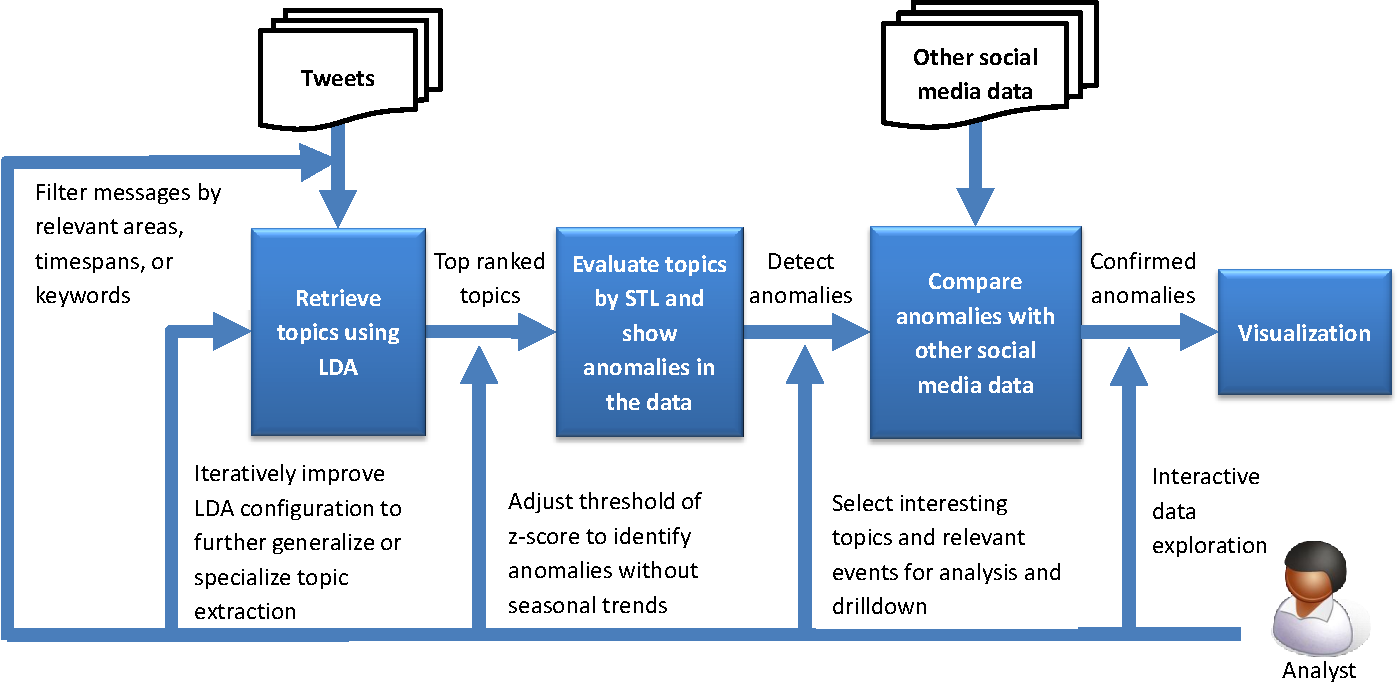
\includegraphics[width=1.0\linewidth]{Overall_Process_crop.pdf}
	\caption{Overview of our iterative analysis scheme for event detection and examination.}
	\label{fig:ad_process}
\end{figure}


\subsection{Social Media Retrieval and Analysis System}
\label{subsec:analysis_system}
Our modular analysis workbench ScatterBlogs was already featured in previous works \cite{Bosch:2011:SGD,Thom:2012:SAD}. 
It proved itself very useful for fundamental tasks like collection, exploration and examination of individual, as well as aggregated, social media messages. The UI of the system is composed of several interconnected views and the main view houses a zoomable openstreetmaps implementation showing message geolocations on a world map. The system features a text search engine and visual content selection tools that can be used to retrieve messages, show spatial and temporal distributions and display textual message contents. Additional visualizations and map overlays provide the analyst with powerful inspection tools, such as a kernel-density heatmap similar to \cite{Maciejewski:2010:VAA}, to show aggregated and normalized message distributions and a movable lens-like exploration tool (called \textquoteleft content lens\textquoteright) that aggregates keyterm frequencies in selected map areas \cite{Bosch:2011:SGD}. To indicate spatiotemporal anomalies in the message set, the system features a mechanism to detect spatiotemporal clusters of similar term usage, and suspicious message clusters can be represented as Tag Clouds on the map \cite{Thom:2012:SAD}. For the real-time collection of messages using the Twitter Streaming API the system features a scalable extraction and preprocessing component. This component was used to collect Twitter messages since August 2011 and it currently processes up to 20 Million messages per day, including the almost complete volume of up to 4 million messages that come with precise geolocation information.

\subsection{Visual Topic Exploration and Event Evaluation}
Results from the topic retrieval and event detection as described in Section~\ref{sec:social_analytics} can be iteratively refined by means of visual result presentation and interactive parameter steering. Both, the final result of event detection as well as intermediary findings during data filtering and topic extraction can be used by the analyst to adjust the process in order to identify interesting topics and keyterms as well as relevant map areas and timespans for a given analysis task. New insights can be generated on each of four individual analysis layers which, in conclusion form an iterative analysis loop from data filtering to result visualization:
\begin{itemize}
	\item \textbf{Spatiotemporal Data Filtering:} The analyst selects an initial spatiotemporal context of Twitter messages to be represented in the visualization and to serve as a basis for analysis. 
He can do so by using textual as well as spatiotemporal query and filter mechanisms that load the relevant base message set from a larger database into active memory. 
The analyst can further filter the base set and remove unimportant parts by using a time-slider, depicting temporal message densities, or polygon and brush selection tools.
% shortened because is prior art
%To filter this base set and to remove unimportant parts, the analyst is provided with an hierarchical time-slider, allowing individual selection of days, hours and minutes. 
%This slider also shows message densities as histograms along the three temporal axis in order to identify high message concentrations. 
%At the same time, polygon and brush selection tools can be applied for spatial filtering.
Using these tools the analyst can gain an initial impression of the spatial and temporal distribution and location of messages that could be relevant for his analysis task.
	\item \textbf{LDA Topic Examination:} In the subsequent step the analyst can choose to start the topic extraction either on the whole analysis context or on some subset of selected messages. At this stage he can utilize the configuration parameters of LDA extraction to interactively explore available topics by generalization and specialization. In this regard the most important parameter is the number of topics that have to be defined for the topic model inference. If the analyst decreases the number using the provided tools, the extracted topics will be more general. If he increases it, they will be more specific and thus candidates for small but possible important events. Once topics are generated from the data they will be presented to the analyst through a list of small tag clouds for each topic. He can now select the topics from the list to see their individual message distribution on the map and the temporal distribution in the time-slider. 
	\item \textbf{STL Evaluation:} Depending on the analyst's choice, the topics can be evaluated and ordered based either on absolute topic frequency or based on abnormality estimates that have been computed using STL. As described in Section~\ref{subsec:filtering}, a valid estimate of abnormality depends on the computation of z-scores from data seven days prior to the observed time frame. Therefore, the STL evaluation will extend the data examination to a range prior to the selected spatiotemporal context, if data is available. Once abnormality is computed for each topic, the topic list will be ordered according to the values and the topics with most outstanding abnormality are highlighted.
	\item \textbf{Crosscheck Validation:} Each selection of messages is accompanied by charts showing the total time series and the remainder components for the selected message set using STL. This is true for spatiotemporal selections as well as for selections using the LDA topic list. In addition to the geolocated Twitter messages this STL is at the same time performed for data that has been extracted from supplemental services like Flickr and YouTube. Based on the multiple charts the analyst can crosscheck the importance and abnormality of examined events and topics.
\end{itemize}


In our system, the analyst is supposed to iteratively use these means of semi-automated processing, visualization and interaction to refine the selection of messages up to a point where he can begin to examine individual message details.
For this task, he can then utilize tools like the content lens for small scale aggregation or the table view to read the messages textual content.
The application of these tools is shown in Figure~\ref{fig:tagcloud}. Usually the most valuable messages will be reports from local eyewitnesses of an important event or from insiders for a given topic. Thus, to retrieve large quantities of such messages helping to understand an ongoing event or situation will be the final goal of the iterative process. Unusual topics, suspicious keyword distributions and events with high STL abnormality discovered on the repeatedly traversed analysis layers can guide the analysis from a very broad and general overview to very specific topics and a relatively small message set suitable for detailed examination.

\begin{figure}[htb]
	\centering
	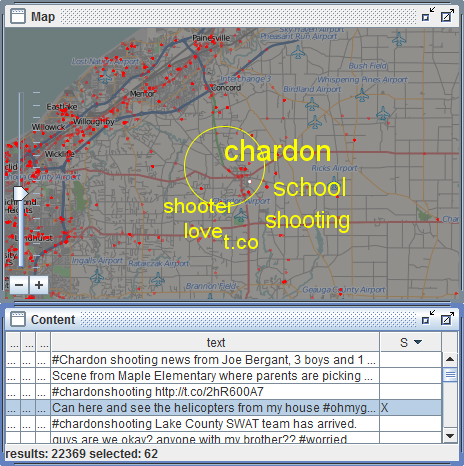
\includegraphics[width=0.6\linewidth]{images/content_investigation}
	\caption{Examining the location of the Chardon high school shooting with a text aggregating content lens.}
	\label{fig:tagcloud}
\end{figure}

\section{Case Study}
\label{sec:case_study}
In this section, we present three case studies for our system covering different types of events including the Chardon High School Shooting, 
the Occupy Wall Street protests in New York, and the 2011 Virginia Earthquake. 
The first case shows how analysts can use our system efficiently to find and explore an abnormal event.
The second case highlights the differences between social media types by cross validation of a planned event.
Finally, the last example showcases the effects of an abrupt, unexpected, natural disaster.

%\begin{figure*}[t]
	%\centering
	%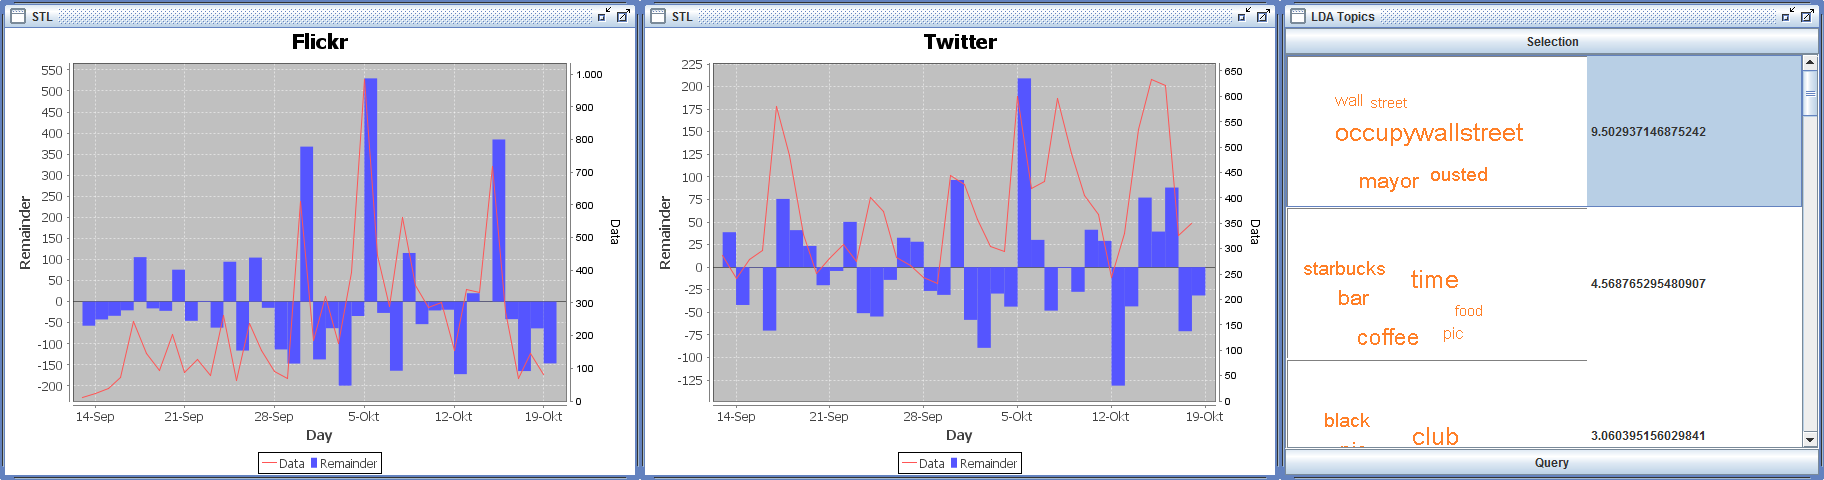
\includegraphics[width=1.00\linewidth]{images/flickrtwitter}
	%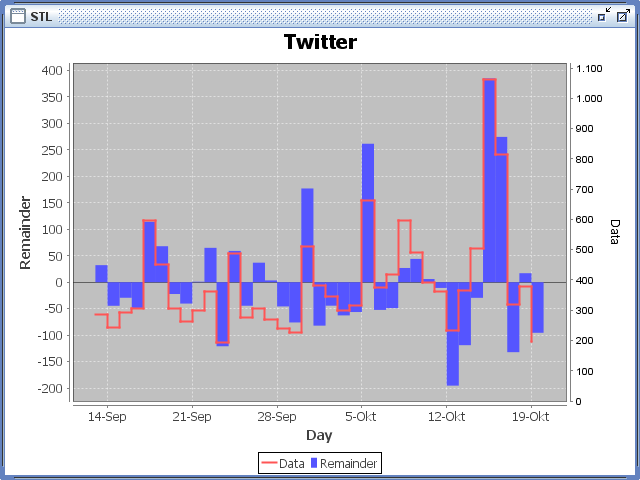
\includegraphics[width=0.45\linewidth]{images/twitter_wallstreet.png}
	%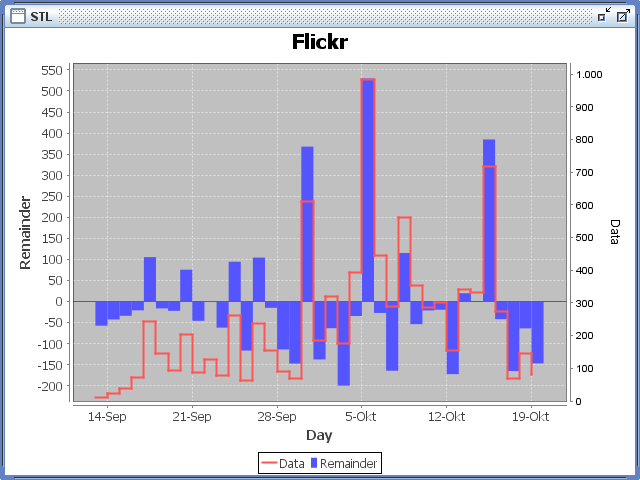
\includegraphics[width=0.45\linewidth]{images/flickr_wallstreet.png}
	%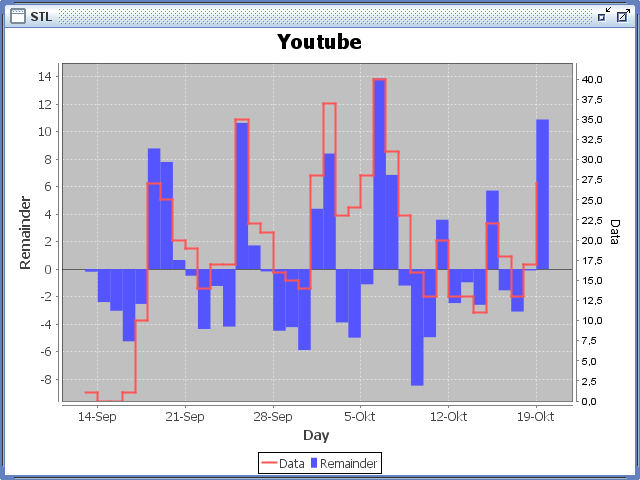
\includegraphics[width=0.45\linewidth]{images/occupyyoutube.png}
	%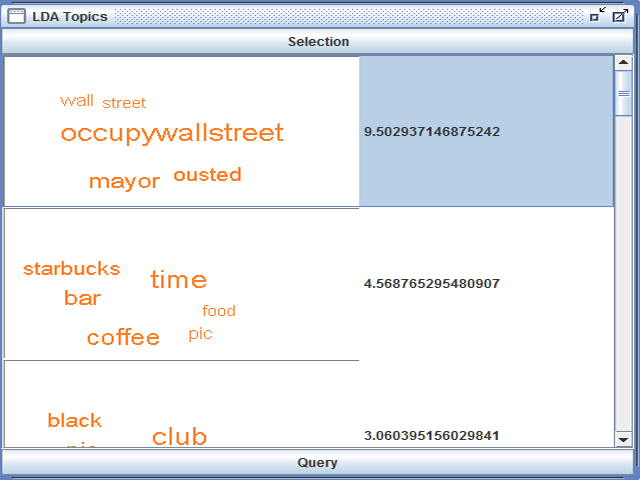
\includegraphics[width=0.45\linewidth]{images/tags_wallstreet.png}
	%\caption{Cross validation of an event using Twitter, Flickr, and YouTube data for the Occupy Wall Street Protests.
	%The protests occurred on Sep. 17 and 30, Oct. 5 and 15. The extracted topics from messages using LDA are displayed with the z-score
	%on the right. The line charts show the remainder components $R_{t}$ (blue) and the original data volumes $Y_{t}=ts_i$ (red) for the STL evaluation.}
	%\label{fig:wallstreet}
%\end{figure*}
	

\subsection{Ohio High School Shooting}
\label{subsec:ohio_shooting}
On February 27, 2012, a student opened fire inside the Chardon High School cafeteria in the early morning.
The gunman killed one student and injured four, from which two eventually died after the incident.

To examine this incident we first locate and select the broader Cleveland area on the map and select a time frame covering three days from February 26 to February 28. 
Using the text search engine and a wildcard query (\textquoteleft *\textquoteright) we can establish an exploration context showing all messages plotted on the map with their respective contents and meta data listed in a separate table view. First, we want to get a broad overview of the topics discussed in the region and thus we select all messages in the area and apply the LDA extraction tool to the current selection. In order to see the most general topics, we chose a low parameter value for the number of topics and a high iteration count to achieve good separation. At this level of semantic detail, the extracted topics indicate messages about the NBA all-star game (February 26 in Orlando) with keywords like \textit{kobe, game, dunk and lebron} as well as the showing of the movie \textquoteleft The Lion King\textquoteright on TV with keywords \textit{king, lion, tv}. If we look at the STL-Diagrams of these topics and the computed z-scores, we also see a peak for these events. By clicking on the retrieved topic representations the associated messages are highlighted in each view. By reading some of the message contents (e.g. \textit{'Watching my fav. Movie on ABC family..... Lion King!!!!', 'Can't wait till the dunk contest starts!'}), the analyst can easily disqualify these from further analysis.

To get a higher semantic resolution we can now increase the number of topics and slightly decrease the iteration count in order to achieve a fast computation. By selecting 20 topics, the topic indicating the shooting event is extracted and indicated by keyterms like \textit{shooting, chardon and school}, alongside the other topics. Although the proportion of the topic is not very high compared to the others, the topic receives a very high z-score (i.e., 3.77) and is ranked among the top five topics (highlighted in orange). Figure~\ref{fig:system} demonstrates the system view of this observation. An analyst can now select the incident topic to see the spatial distribution of associated messages on the maps as well as the temporal distribution in the timeslider histogram. By examining messages using the content lens to aggregate topics over map areas as well as the tools for reading individual message contents, we can easily distinguish between messages informed by media reaction and messages of actual observers in the Chardon High School area. In this case, after isolating the messages from local observers, we find messages like \textit{\textquoteleft Omg shooting at Chardon High School?!?!\textquoteright} and \textit{\textquoteleft Helicopter overhead. We are on scene. Message from school says students moved to middle school\textquoteright}.

\begin{figure}[tb]
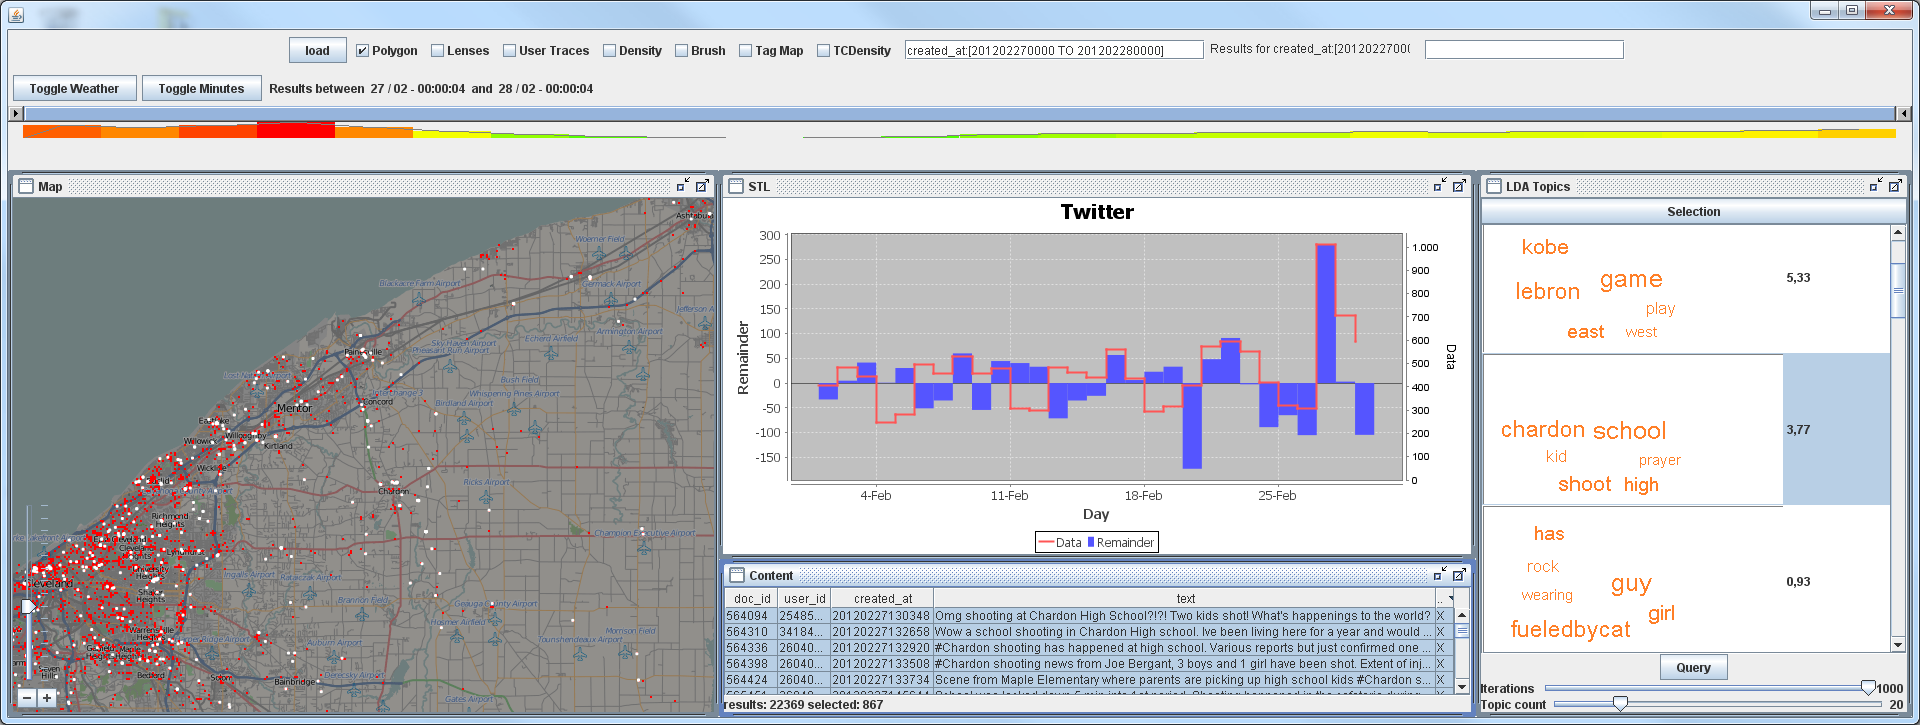
\includegraphics[width=1.0\linewidth]{teaser}
\caption{Social media analysis system including message plots on a map, abnormality estimation charts and tables for message content and topic exploration. 
  It can be seen, how the Ohio High School Shooing on February 27, 2012 is examined using the system. The selected messages, marked as white dots on the map, show retrieved Tweets that are related to the event.}
\label{fig:system}
\end{figure}



%To discussion -> Athough the detected messages could help to identify local witnesses of some event, the frequencies of messages with geocoordinates are still very low in moderately populated areas ---- daher könnte man die Nützlichkeit zum gegenwärtigen Zeitpunkt sicher hinterfragen...

%\footnote{\url{http://www.cbsnews.com/8301-504083_162-57386775-504083/third-chardon-high-school-shooting-victim-demetrius-hewlin-dies/}}

\subsection{Occupy Wall Sreet}
\label{subsec:occupy_wallst}

Starting on September 17, 2011 in the Wall Street financial district in New York City,
people have been gathering for the Occupy Wall Street protest movement.
The movement against economic inequality has since spread to other major cities throughout the world.
Various social media services including Twitter, Facebook, Flickr and Youtube have been utilized both by the participants and the global media for communication and reports about the movement in forms of text, images and videos. 
For the related extracted topic (\textit{occupywallstreet, wall, takewallstreet, takewallst, park}), 
Figure~\ref{fig:wallstreet} shows the results of our abnormality estimation for the three social media services Twitter, Flickr, and YouTube over the course of one month.
As shown in Figure~\ref{fig:plot}, in each of the marked regions, at least two of the services show z-scores over 2.0 and they correspond to actual events during the Occupy Wall Street protests.
From this experimental result, one can derive a strong correlation between the three social media data sources.
The related data volumes and remainder ($R$) are shown in Figure~\ref{fig:wallstreet} for all three providers.

\begin{figure}[tb]
\centering
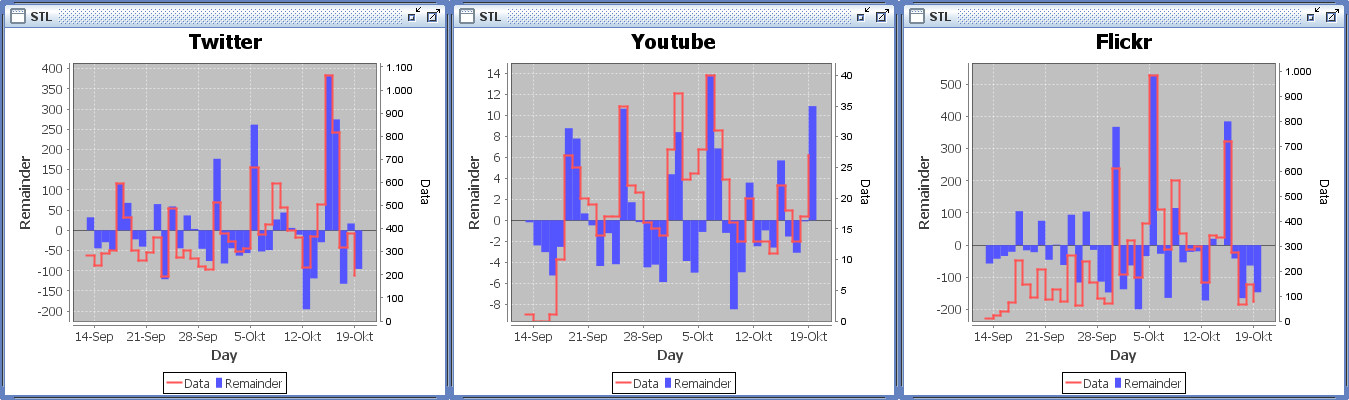
\includegraphics[width=1.0\linewidth]{crosscompare_new}
\caption{Cross validation of an event using Twitter, Flickr, and YouTube data for the Occupy Wall Street Protests.
	The protests occurred on Sep. 17 and 30, Oct. 5 and 15. The line charts show the remainder components $R$ (blue) and the original data volumes $Y$ (red) for the STL evaluation. The scales on the right and left side of each chart view are adapted to the maximum values.}
\label{fig:wallstreet}
\end{figure}


\begin{figure}[tb]
\centering
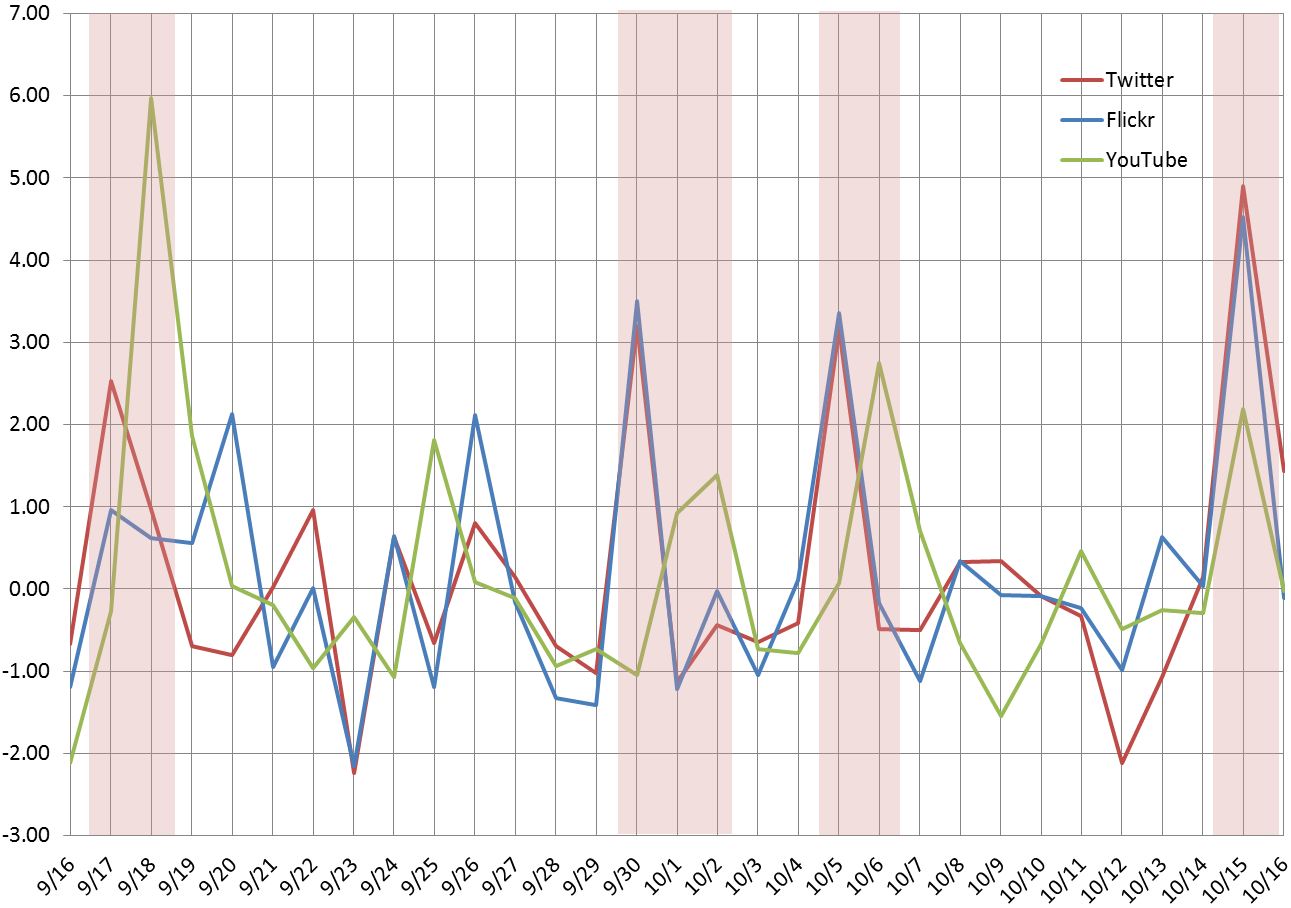
\includegraphics[width=0.8\linewidth]{z-score-plot}
\caption{Abnormality and correlation on multiple social media sources. 
As a result of high z-scores around the same time periods, we found a strong correlation 
between the three social media sources. Marked regions correspond to periods where at least 2 providers received scores over 2.0.}
\label{fig:plot}
\end{figure}



As shown in Figure~\ref{fig:plot}, on September 17 (the first day of the protests with approximately 1,000 participants~\cite{Sept17}),
only the Twitter stream received an abnormal score while the Flickr and YouTube data artifacts are delayed by 1-3 days.
We attribute this initial delay to the simple nature of Twitter usage compared to Flickr and YouTube where the data potentially has to be recorded, edited, and uploaded and is thus more labor intensive.
Additionally, eighty protesters where arrested while marching uptown on September 24, but even though Flickr and YouTube reaction on this event created higher z-scores in the following days, they were not significant enough to register an event.
The following spikes of high z-scores overlap with a march across the Brooklyn Bridge (Oct. 1~\cite{Oct01}), a large demonstration (Oct. 5~\cite{Oct05}), and globally coordinated protests (Oct. 15~\cite{Oct15}).

%For YouTube, the high abnormalities usually come with a delay between one and two days.
%Our system found the additional abnormal events \textit{oakland, tear, gas, general, san}~\cite{Duell:2011:OOI} and \textsl{bridge, brooklyn, arrests, march, police}~\cite{Chiaramonte:2011:CMO} in the YouTube meta-data, which were not detectable in Twitter and Flickr.
%Our system also provides further analysis on YouTube data. 
%We applied our abnormality estimation method to meta-data from YouTube. 
%Our system additional found more abnormal events;

%%
%% Table of experimental results of topic model
%%
%\begin{table}\footnotesize
%\begin{table}
%\small
%\centering
%\begin{tabular}{|l|c|c|c|}
%	\hline
%	 Date & Twitter & Flickr & YouTube \\
%	\hline\hline
%%	Sep. 16, 2011 & -0.67 & -1.19 & -2.12 \\
%	Sep. 17, 2011 & \textbf{2.53} & \textbf{0.97}& \textbf{-0.26} \\ %& The protests movement began \\
%	Sep. 18, 2011 & 0.97 & 0.62 & 5.98 \\ 
%	Sep. 19, 2011 & -0.69 & 0.56 & 1.86 \\
%	Sep. 20, 2011 & -0.80 & 2.13 & 0.04 \\
%	Sep. 21, 2011 & 0.02 & -0.95 & -0.19 \\
%	Sep. 22, 2011 & 0.96 & 0.01 & -0.96 \\ 
%	Sep. 23, 2011 & -2.24 & -2.15 & -0.34 \\
%	Sep. 24, 2011 & 0.63 & 0.64 & -1.07 \\
%	Sep. 25, 2011 & -0.66 & -1.19 & 1.81 \\
%	Sep. 26, 2011 & 0.80 & 2.11 & 0.08 \\
%	Sep. 27, 2011 & 0.14 & -0.16 & -0.11 \\
%	Sep. 28, 2011 & -0.70 & -1.32 & -0.94 \\
%	Sep. 29, 2011 & -1.02 & -1.41 & -0.73 \\
%	Sep. 30, 2011 & \textbf{3.20} & \textbf{3.50} & -1.05 \\%& Big movement \\
%	Oct. 1, 2011 & -1.14 & -1.22 & 0.92 \\
%	Oct. 2, 2011 & -0.44 & -0.03 & \textbf{1.38} \\
%	Oct. 3, 2011 & -0.64 & -1.05 & -0.73 \\
%	Oct. 4, 2011 & -0.42 & 0.11 & -0.77 \\
%	Oct. 5, 2011 & \textbf{3.17} & \textbf{3.36} & 0.07 \\ %& Unions, students join the protest\\
%	Oct. 6, 2011 & -0.49 & -0.18 & \textbf{2.75} \\
%	Oct. 7, 2011 & -0.50 & -1.12 & 0.7 \\
%	Oct. 8, 2011 & 0.32	& 0.34 & -0.65 \\
%	Oct. 9, 2011 & 0.34	& -0.07 & -1.54 \\
%	Oct. 10, 2011 & -0.09 & -0.08 & -0.67 \\
%	Oct. 11, 2011 & -0.33 & -0.23 & -0.46 \\
%	Oct. 12, 2011 & -2.12 & -0.99 & -0.49 \\
%	Oct. 13, 2011 & -1.07 & 0.63 & -0.26 \\
%	Oct. 14, 2011 & 0.15 & 0.04 & -0.3 \\
%	Oct. 15, 2011 & \textbf{4.90} & \textbf{4.53} & \textbf{2.19} \\ %& Global day of action \\
%%	Sep. 17, 2011 & 2.53 & 0.97 & Sep. 18, 2011 & 5.98 \\ %& The protests movement began \\
%%	Sep. 30, 2011 & 3.20 & 3.50 & Oct. 2, 2011 & 1.38 \\%& Big movement \\
%%	Oct. 5, 2011 	 & 3.17	& 3.36 & Oct. 6, 2011 & 2.75 \\ %& Unions, students join the protest\\
%%	Oct. 15, 2011   & 4.90 & 4.53 & Oct. 15, 2011 & 2.19 \\ %& Global day of action \\
%	\hline
%\end{tabular}
%\caption{Abnormality and correlation on multiple social media. 
%As a result of the high z-scores around the same time, we found a strong correlation 
%between the three social media sources.}
%\label{T:Correlation}
%\end{table}
%\footnote{\url{http://www.nytimes.com/2011/11/25/business/media/occupy-movement-focuses-on-staying-current-on-social-networks.html}}

%\subsection{2011 Virginia earthquake}
%\label{subsec:virginia_earthquake}
%A magnitude 5.8 earthquake occurred on August 23 afternoon, 2011 in Mineral, Virginia,
%according to the U.S. Geological Survey\footnote{\url{http://earthquake.usgs.gov/earthquakes/recenteqsww/Quakes/se082311a.php}}.
%During and after the tremors were felt along the East Coast,
%Twitter users posted more than 40,000 earthquake-related reaction tweets
%within a minute of its occurrence\footnote{\url{http://mashable.com/2011/08/23/virginia-earthquake/}}.
%There are some example Twitter messages;
%\textit{EARTHQUAKE!!!!!!!}; \textit{Whoa!!!! Just experienced an earthquake here in Virginia!!!!}; 
%\textit{Omg I just felt an earthquake}.
%Using our method, we found also the z-score of the topic indicating the earthquake event was 
%extremely high (i.e., 10.63).
\subsection{2011 Virginia Earthquake}
\label{subsec:virginia_earthquake}
For the last use case we examine a magnitude 5.8 earthquake that occurred on the afternoon of August 23rd 2011 in Mineral, Virginia~\cite{USGS:2011:M5V}.
%\footnote{\url{http://earthquake.usgs.gov/earthquakes/recenteqsww/Quakes/se082311a.php}}.
Starting with the minute of the earthquakes occurrence, Twitter users posted more than 40.000 earthquake-related Tweets reporting tremors they felt along the East Coast~\cite{Indvik:2011:ECT}.
%\footnote{\url{http://mashable.com/2011/08/23/virginia-earthquake/}}.
Among these were messages like:
\textit{\textquoteleft EARTHQUAKE!!!!!!!\textquoteright}; \textit{\textquoteleft Whoa!!!! Just experienced an earthquake here in Virginia!!!!\textquoteright}; and 
\textit{\textquoteleft Omg I just felt an earthquake\textquoteright}.
Figure~\ref{fig:earthquake} gives an impression how our system is applied to examine this event.

\begin{figure}[htb]
	\centering
	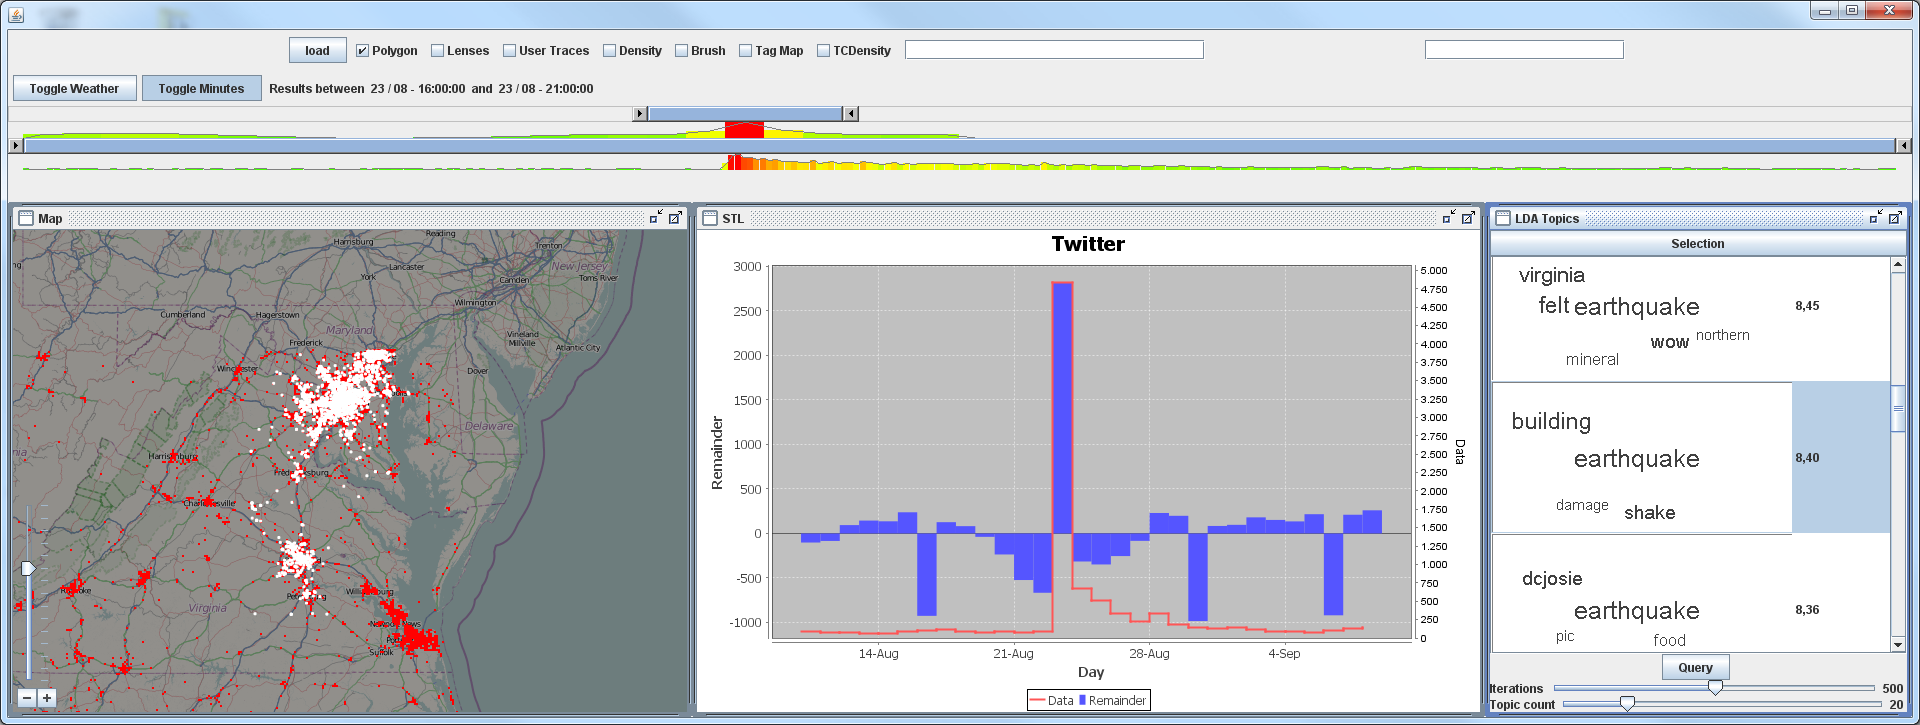
\includegraphics[width=1.0\linewidth]{earthquake3}
	\caption{Virginia earthquake on August 23rd, 2011. Our abnormal event detection system detects the earthquake event
	using our STL based anomaly detection algorithm. The abnormality degree is extremely high
	on August 23rd, 2011 (times are given in UTC).}
	\label{fig:earthquake}
\end{figure}

For the analysis we begin with selecting the Virginia area from Baltimore to Virginia Beach and three days around the 23th. A topic extraction with 5 topics and just 100 iterations already retrieves two earthquake related topics showing that this event is very prominent within the selection. By clicking these topics one can observe that the highest density of earthquake messages can be found in the Washington, Baltimore and Richmond areas. 

To observe the areas in more detail we combine the topic selection with a spatial selection of the three cities and reapply the topic extraction. This time we use 20 topics with 500 iterations. Since we are now operating only on earthquake related messages, the retrieved topics all contain earthquake as a dominant keyword. On this level of detail we can see topics indicating that buildings have been evacuated due to the earthquake (\textit{earthquake, people, evacuated, early, building}) and that damage has been caused (\textit{earthquake, building, shake, damage}). The z-scores for all top ranked topics are now very high (often above 8.0) and thus indicate the high abnormality of this event. 

Finally, when going into even higher detail with 100 topics and 1000 iterations we can see smaller events within the big earthquake event. For example, one topic indicates that damage was caused to the Washington Monument and by clicking on the topic we can see messages like \textit{\textquoteleft damage to Washington Monument\textquoteright}; \textit{\textquoteleft Washington Monument is tilting?!? \textquoteright}; and \textit{\textquoteleft Helicopter just landed next to Washington Moniment, west side. \#DCearthquake \textquoteright}. There are also misleading messages, indicating that the damage to the Washington Monument was just false rumors: \textit{\textquoteleft the Washington monument was not damaged in any way from the earthquake. \#rumor\textquoteright}. However, media crosschecks show that visible damages did in fact happen and will probably cost the city 15 million dollars to repair~\cite{Huffingtonpost:2012:Web}.

At this point, it is important to note, that while several earthquake topics produced significant z-values in Twitter, the event did not produce high z-scores in Flickr and YouTube.
This is probably due to fact, that many people will write a quick message after a shock has been felt by themselves, but it takes quite some time until images or videos are uploaded from cameras to Flickr and YouTube. The event also demonstrates that large and unexpected events will produce immediate and significant reactions in services like Twitter and they can thus easily be detected by using our system.

\section{Discussion}
\label{sec:disc}
In this section we want to discuss four important notes and observations relevant to the presented approach.

\textbf{Event Types:} As was demonstrated with the three case studies, events in social media can be categorized into two different types. 
The 2011 Virginia Earthquake and the Ohio High School Shooting can be categorized as abrupt or disaster events,
while Occupy Wall Street can be considered a social and planned event.
The two types of events have quite distinguishable features.
For the abrupt events, there is a strong change in daily counts mainly in the text based Twitter messages.
For the planned event, the Twitter signal may still be faster, but due to the gradual increase and decrease, it is less pronounced.
In contrast, Flickr and YouTube have delayed, but very prominent changes, for planned events; 
however, we could not find significant signals for abrupt events.
This reflects that video and photo recording happen rarely during abrupt events.
Social events, e.g., Occupy Wall Street or election debates, however, have a high impact on such multimedia based social media; 
Relevant videos, photos, and even meta-data (e.g., descriptions, tags) allow analysts to find additional information about them.
We, therefore, think that cross validating events among multiple social media types is important in order to establish situational awareness.

\textbf{Base Data:} Regarding the base data, it is important to note, that our approach depends on geo-located Twitter messages with precise coordinates, which are only a fraction of the whole Twitter stream.
While this fraction still consists of several million messages per day, 
it is not a representative sample of the population, because it mainly covers mobile users equipped with GPS enabled devices.
We think, however, that mobile users, who share their daily experiences freely, are the most relevant group for situational awareness scenarios.
Some studies~\cite{Cheng:2010:YYT, Jalal:2012:WIT} tried to overcome the problem of location information scarcity in Twitter messages, which adds another source of uncertainty.
First, the user's self reported locations can be outdated.
Second, the geo-coding of the location can be considerably wrong due to place name ambiguities.
Furthermore, we have just shown the feasibility of the approach for Twitter, Flickr, and YouTube data, but it can easily be adapted to other social media providers like Facebook or Forsquare as well, in order to widen the sample of the population.

\textbf{Probabilistic Models:} In this work, we use STL to decompose time series of topic streams.
There are many alternative statistical models for this task, such as DHR (Dynamic Harmonics Regression)~\cite{Young:1999:DHR} and SARIMA (Seasonal AutoRegressive Intergrated Moving Average)~\cite{Box:1990:TSA}.
DHR and SARIMA models are particularly useful for forecasting and STL can also be used for prediction based on seasonal (periodic) time series~\cite{Jiang:2010:MML}.
Our main reasons for choosing STL was the fact that it is non-parametric, can be computed faster than SARIMA~\cite{Jiang:2010:MML} and needs less training data for equally good results.

\textbf{End User Feedback:} We requested informal feedback from users within our institutes and received comments and suggestions. 
To compare the LDA topic modeling plus the seasonal-decomposition based abnormality analysis versus only the LDA topic modeling, we enabled our system to switch between these modes. 
The users were impressed by the fact that both results (two lists of topics) from two different modes were quite different. 
Highly ranked topics by LDA topic modeling consisted of ordinary words, while the combined analysis was indicating unusual events. 
They noted that the tightly integrated visual analysis workbench was useful to apply the automated methods. 
Furthermore, they suggested a function allowing people to see a pattern of abnormality for a user-defined topic.

\section{Summary}
\label{sec:concl}
We presented an interactive abnormal event detection and examination system for the analysis of multiple social media data sources.
The system uses an abnormality estimation scheme based on probabilistic topic modeling and seasonal-trend decomposition to find and examine relevant message subsets. This scheme is tightly integrated into an highly interactive visual analytics system, which supplements tools based on automated message evaluation with sophisticated means for parameter steering, filtering and aggregated result set exploration.
Three use cases demonstrated the visualization and user interaction within the system and its capabilities to detect and examine several different event types from social media data.
The ability to crosscheck findings based on three distinct social media sources revealed the kinds of correlations that can be expected from various event types.
%Finally, we showed that our interactive system allows an effective analysis of a massive social media data set.

%For future work, we will further investigate context-based analysis and improve the current detection algorithm to allow for a faster analysis.
%Due to the fast-paced and low quality nature of microblogging, we will also investigate the effects of additional preprocessing options like automated spell-checking or synonym recognition under the constraint of preventing ambiguities.
%Furthermore, we want to supplement the system with real-time monitoring features, demanding additional means for adaptive attention guiding as well as interaction techniques for use in high pressure environments. For the final system we are currently preparing a thorough evaluation to test it in cooperation with crisis management personnel and other domain experts.


